\documentclass[14pt,aspectratio=1610]{beamer}
\usepackage[utf8]{inputenc}
\usepackage[ngerman]{babel}
\uselanguage{ngerman}
\languagepath{ngerman}
\usetheme{simple}
\usecolortheme{whiteonblack}
\usepackage{array}
\usepackage{aurl}
\daurl{meta}{http://www.snik.eu/ontology/meta/}
\daurl{ob}{http://www.snik.eu/ontology/ob/}
\daurl{bb}{http://www.snik.eu/ontology/bb/}
\usepackage{url}
\usepackage{graphicx}
\usepackage{csquotes}
\usepackage{amssymb}
\usepackage{pifont}
\newcommand{\xmark}{\ding{55}}%
\newcolumntype{H}{>{\setbox0=\hbox\bgroup}c<{\egroup}@{}} % comment out columns
%\date{25. März 2022}
%\author{\texorpdfstring{Konrad Höffner\newline\url{konrad.hoeffner@imise.uni-leipzig.de}}{Konrad Höffner}}
\title{SHACL}
\subtitle{Shapes Constraint Language}
\begin{document}

\begin{frame}
\titlepage
\end{frame}

\begin{frame}{}
\centering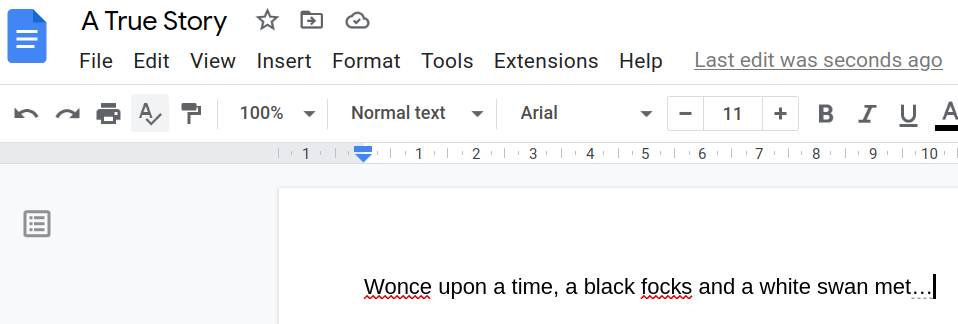
\includegraphics[width=1.05\textwidth,height=1.05\textheight,keepaspectratio]{img/spelling.png}
\end{frame}

\begin{frame}{}
\centering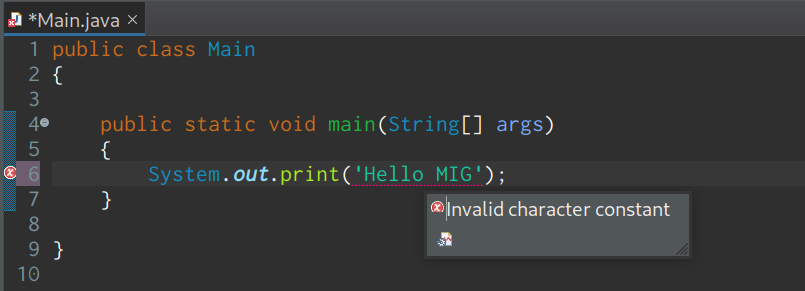
\includegraphics[width=1.05\textwidth,height=1.05\textheight,keepaspectratio]{img/javaerror.png}
\end{frame}

\begin{frame}{}
\centering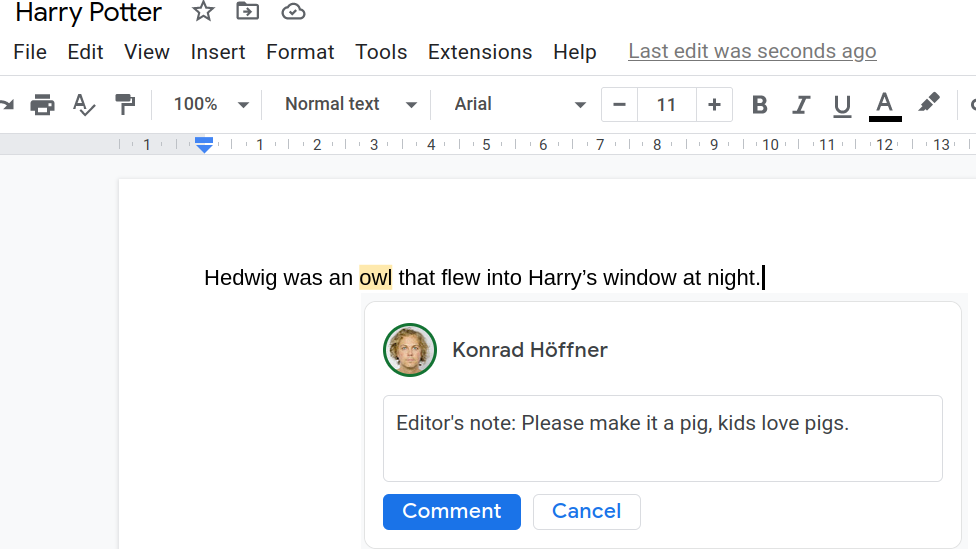
\includegraphics[width=1.05\textwidth,height=1.05\textheight,keepaspectratio]{img/hedwig.png}
\end{frame}

\begin{frame}{}
\centering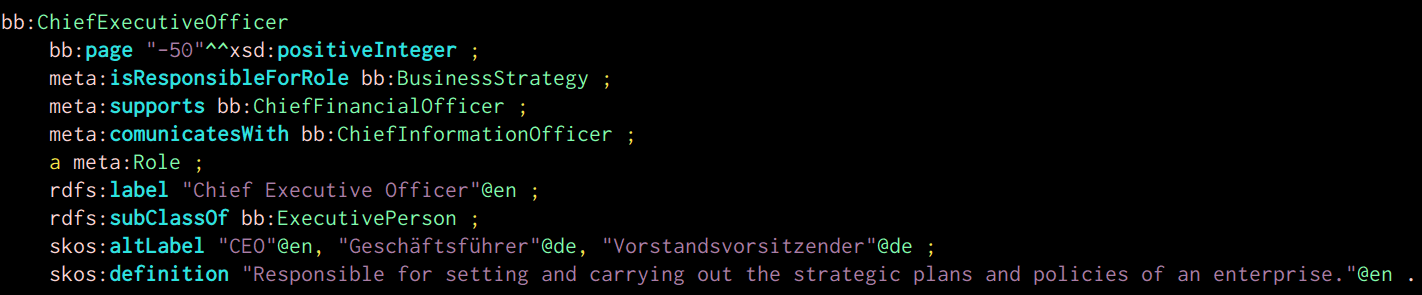
\includegraphics[width=1.05\textwidth,height=1.05\textheight,keepaspectratio]{img/bb-ceo.png}
\end{frame}

\begin{frame}{}
\centering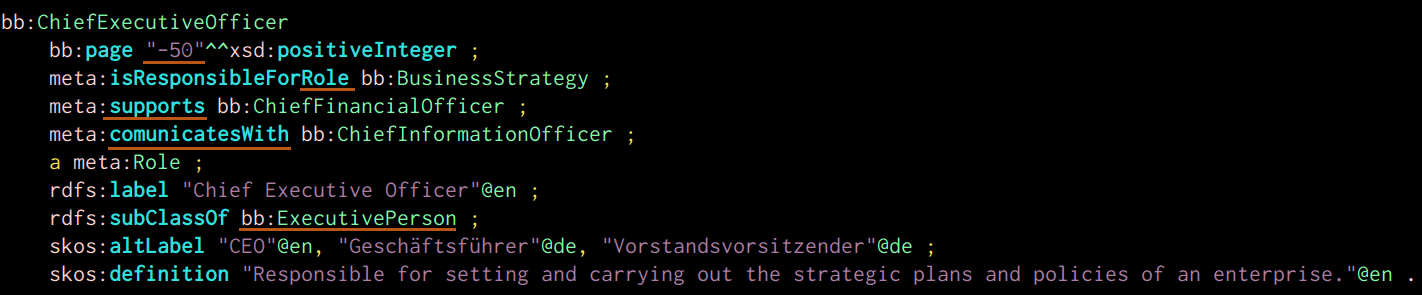
\includegraphics[width=1.05\textwidth,height=1.05\textheight,keepaspectratio]{img/bb-ceo-marked.png}
\end{frame}

\begin{frame}{bla}
\centering\includegraphics[width=1.05\textwidth,height=1.0\textheight,keepaspectratio]{img/SNIK_Metamodell_V8.pdf}
\end{frame}

\begin{frame}[fragile]{}
\begin{verbatim}
:Role
    a owl:Class ;
    rdfs:label "Rolle"@de, "role"@en ;  
    rdfs:subClassOf :Top ;
    owl:disjointWith :EntityType, :Function .

:communicatesWith
    a owl:ObjectProperty ; 
    rdfs:domain :ApplicationComponent ;
    rdfs:label "communicates with"@en, "kommuniziert mit"@de ;
    rdfs:range :ApplicationComponent .
}
\end{verbatim}
\end{frame}

\begin{frame}{Problem}
\begin{itemize}
\item $\ldots$
\end{itemize}
\end{frame}

\end{document}
